\documentclass[11pt,a4paper]{article}
\usepackage[left=2cm,text={17cm,24cm},top=3cm]{geometry}
\usepackage[slovak]{babel}
\usepackage[]{opensans}
\usepackage[utf8]{inputenc}
\usepackage[T1]{fontenc}
\usepackage{graphicx}
\graphicspath{{.}}
\usepackage{times}
\usepackage{cite}
\usepackage{url}
\usepackage{enumitem}
\usepackage{indentfirst}
\usepackage{color}
\usepackage[unicode,colorlinks,hyperindex,plainpages=false,urlcolor=black,linkcolor=black,citecolor=black]{hyperref}
\usepackage{xcolor}
\usepackage{listings}
\lstset{basicstyle=\ttfamily,
  showstringspaces=false
}

\providecommand{\uv}[1]{\quotedblbase #1\textquotedblleft}

\clubpenalty=10000
\widowpenalty=10000

\begin{document} %#################################################################################

%TITLEPAGE
\begin{titlepage}

\begin{center}

	\thispagestyle{empty}

	\textsc {
		\Huge Vysoké učení technické v~Brně\\[0.4em]
		\huge Fakulta informačních technologií
	}\\

	\vspace{\stretch{0.382}}

	{
		\LARGE Sieťové aplikácie a správa sietí\\[0.4em]
		\Huge POP3 server
	}

	\vspace{\stretch{0.618}}

\end{center}

	{
		\LARGE \today \hfill Adrián Tóth
	}

\end{titlepage}	

%CONTENT
\setlength{\parskip}{0pt}
{\hypersetup{hidelinks}\tableofcontents}
\setlength{\parskip}{0pt}

\newpage %#########################################################################################

\section{Úvod}
	\indent Projekt sa vzťahuje k predmetu \textit{ISA - Sieťové aplikácie a správa sietí}, kde je úlohou naimplementovať \textbf{\textit{POP3 server}}, ďalej označovaný ako \textit{server}. Server je naimplementovaný podľa RFC 1939\cite{POP3} ktorý využíva \textit{BSD sockets} na komunikáciu.\\
	\indent Server pracuje so súbormi v jednom priečinku, ktorý sa nazýva maildir. Maildir\cite{MAILDIR} je priečinok, ktorý obsahuje ďalšie podpriečinky \textit{new}, \textit{cur} a \textit{tmp}. Všetky súbory v priečinku maildir by mali byť vo formáte IMF podľa RFC 5322\cite{IMF}.\\
	\indent Server využíva okrem maildiru ešte jeden súbor a to kvôli autentifikácii užívateľa v ktorom sú uložené prihlasovacie údaje. Potrebné informácie, ktoré si server potrebuje uchovať, ukladá do logovacích súborov ktoré sa uložia do toho priečinka v ktorom je server spustený.

\section{Pojmy}

	\subsection{Maildir}
		\indent Maildir označuje priečinok ktorý server využíva k svojmu behu. Maildir je zadaný hneď pri spustení po parametri \uv{-d} a to cestou ku priečinku. Priečinok môže byť zadaný absolútnou cestou alebo relatívnou. Maildir slúži na ukladanie správ (súborov) užívateľa do podpriečinkov podľa určitých kritérii. Maildir obsahuje podpriečinky \textit{cur}, \textit{new} a \textit{tmp}. Súbory sa nachádzajú v podpriečinku new, ak sú označené ako nová správa. Po pripojení klienta sa presunú do podpriečinku cur. Priečinok cur obsahuje všetky správy, ktoré boli najskôr v priečinku new ale po pripojení klienta sa presunuli do tohto priečinka. Odstránenie správ z priečinka cur je záležitosť klienta. Priečinok tmp slúži ako dočasné úložisko pre server.

	\subsection{IMF}
		\indent Internet Message Format v skratke IMF definuje formát správy ako je uložená v súbore. Definuje správu ako sekvenciu znakov tvoriace riadky, ktoré sú ukončené s dvoma znakmi a to carriage-return a line-feed. Carriage-return označovaný ako CR je znak \uv{\textbackslash r} a line-feed označovaný ako LF je znak \uv{\textbackslash n}. Takže správa je vlastne množina riadkov, ktoré sú sekvencia po sebe idúcich znakov, kde každý riadok je ukončený s dvoma znakmi CRLF.

	\subsection{POP3}
		\label{fig:pop3}
		\indent Pojem POP3 označuje Post Office Protocol - Version 3\cite{POP3} čo je internetový protokol aplikačnej vrstvy používanie na správu emailov. Tento protocol definuje pomocou množín noriem a pravidiel spôsob komunikácie s pop3 serverom a funkcionalitu tohto servera na ktorom je spustený. Tento protokolom definovaný server slúži k správe e-mailov a ich prenos medzi serverom a klientom.\\[0.4em]
		Server je riadený jedným rozsiahlejším konečným automatomatom. Protokol špecifikuje jednotlivé stavy konečného automatu a príkazy ktoré určujú prechody medzi nimi, konečný automat môžete vidieť v prílohe na obrázku číslo \ref{IMG-FSM}. Z obrázku je zrejmé že pri pripojení klienta je počiatočný stav \textit{authorization} kde sa čaká na autentifikáciu pomocou príkazov APOP alebo USER a PASS. Následne po autentifikácii sa uzamkne priečinok maildir a ostatný klienti musia počkať až kým sa pripojený klient neodpojí. Po autentifikácii sa server nachádza v stave \textit{transaction}. V tomto stave môže spravovať správy uložené na serveri pomocou príkazov RSET, STAT, LIST, UIDL, RETR, DELE. V tomto stave sú ešte ďalšie dva príkazy a to NOOP, ktorý nevykoná nič, a QUIT, ktorý ukončí spojenie s klientom a presunie server do stavu \textit{update}. Server v stave \textit{transaction} nevykoná žiadnu zmenu nad súbormi, ale po presune do stavu \textit{update} vykoná všetky klientom zadané zmeny nad maildirom, napríklad vymaže súbor z disku. Na konci stavu \textit{update} sa odomkne maildir ktorý už obsahuje zmeny vykonané odhláseným klientom a čaká sa na ďalšieho klienta ktorý sa bude chcieť pripojiť.\\[0.4em]
		Server vždy reaguje na príkazy prijaté od klienta dvojakým spôsobom, a to buď odošle pozitívnu odpoveď vo forme \uv{+OK ...} alebo negatívnu odpoveď \uv{-ERR ...}. Negatívna odpoveď obsahuje popis vzniknutej chyby a popis pozitívnej odpovede je definovaný v protokole POP3\cite{POP3}.


\section{Návrh a implementácia}

	\indent K implementácii bol zvolený viacparadigmatový programovací jazyk C++, pretože umožňuje objektovo orientované programovanie. V ďalších podkapitolách bude popísaná samotná implementácia POP3 servera, ktorá popisuje projekt z hľadiska implementácie funkcionality tohto servera, t.j. ako je program delený na logické časti, ktoré zaručujú určitú časť funkcionality servera a spolu nasledujúc po sebe tak zaručujú správny beh programu.

	\subsection{Moduly}
		
		\indent Projekt bol rozdelený na moduly, ktoré tvoria určité logické celky.

		\begin{itemize}

			\item \textit{constatns}\\[0.4em]
				\label{fig:uid}
				Modul obsahujúci konštanty. Tu sa nachádza aj konštanta, ktorá reprezentuje znakovú sadu z ktorej sa generuje \textit{unique-id}. Podľa RFC 1939 \textit{unique-id} pozostáva z ASCII znakov od 0x21 do 0x7E. Server však podporuje všetky tieto znaky, okrem znaku 0x2F, t.j. znak \uv{ / }. Znak \uv{ / } sa využíva ako oddeľovací znak v logovacích súboroch. V tomto module sa nachádzajú aj konštanty určujúce veľkosti, názvy.

			\item \textit{argpar}\\[0.4em]
				Modul obsahujúci funkciu na parsovanie vstupných parametrov, funkciu na vypísanie \uv{help} správy na stdout a funkciu na načítanie prihlasovacích údajov zo súbora. Funkcia argpar v závislosti od parametrov inicializuje lokálnu premennú args v popseri. S premennou args sa často pracuje, pretože obsahuje všetky informácie, ktoré sú potrebné k behu programu. Premenná je objekt vytvorený z triedy Args definovaný v module datatypes.

			\item \textit{checks}\\[0.4em]
				Modul obsahujúci funkcie, ktoré slúžia na kontrolu im predaných parametrov.

			\item \textit{datatypes}\\[0.4em]
				Modul obsahujúci mnou definované enumeračné premenné, triedu Args spomenutú v predošlom bode \uv{\textit{argpar}} a ešte jednu funkciu. Enumeračné premenné sa používajú v automate, kde označujú stav alebo príkaz, ktorý sa nachádza v module fsm. Trieda Args slúži na posun informácii medzi funkciami pričom je inicializovaná hned na začiatku spustenia programu funkciou argpar. Funkcia, ktorá sa nachádza v tomtot module slúži na transformáciu vstupného reťazca na výstupný k nemu vzťahujúcu sa enumeračnú hodnotu typu Command.

			\item \textit{fsm}\\[0.4em]
				Modul nazýva ako \uv{finite-state machine}, skrátene fsm, obsahuje samotnú implementáciu konečného automatu podľa RFC 1939. Modul reprezentuje funkcionalitu jedného vytvoreného vlákna, ktoré obsluhuje napojeného klienta. Obsluha klienta je naimplementovaná ako konečný automat vo funkcii \uv{thread\_main}. V tejto funkcii sa nachádza všetko potrebné, aby sa správne obslúžil pripojený klient, odpojil a aby sa vykonali ním požadujúce zmeny. Taktiež sa tu nachádzajú funkcie, ktoré vypomáhajú konečnému automatu.

			\item \textit{logger}\\[0.4em]
				Modul obsahujúci všetky ostatné funkcie, ktoré sú prevažne volané z fsm a z argpar. Nachádzajú sa tu funkcie ktoré vykonávajú logovanie informácii do súboru a prácu nad týmito informáciami. Taktiež sa tu nachádza funkcia reset.

			\item \textit{md5}\\[0.4em]
				Modul ktorý obsahuje oddelenú časť zodpovednej za generovanie MD5 hashu pre príkaz APOP. Tento hash sa generuje zo špecifického typu reťazca, ktorý sa nazýva podľa RFC 1939 ako \uv{greeting banner}. Zodpovedná funkcia na generovanie tohto reťazca sa tu tiež nachádza.

			\item \textit{popser}\\[0.4em]
				Hlavná časť programu, kde sa volajú všetky ostatné moduly. Tu sa nachádza aj hlavná funkcia \uv{main}. V tejto časti, po spracovaní parametrov, sa vytvorí komunikácia a pri úspešnom pripojení klienta sa vytvorí vlákno, ktorému je predaná funkcia \uv{thread\_main} a soket na ktorom sa pripojil klient. Taktiež sa tu nachádza odchytávanie signálu SIGINT, čo má za následok správne ukončenie celého servera.

		\end{itemize}

	\subsection{Inicializácia, Spracovanie parametrov, Naviazanie komunikácie}
		\indent Pri prvom spustení servera sa vytvoria pomocné globálne premenné, ktoré budú riadiť beh celého procesu. Proces využíva tri globálne premenné z ktorých sú dve premenné typu \textit{bool} a zvyšná premenná typu \textit{std::mutex}.\\[0.4em]
		\indent Prvým krokom je spracovanie parametrov a inicializácia objektu typu Args ktorý nesie všetky potrebné informácie obsiahnuté z parametrov a následne sa predáva ďalším funkciám. Túto incializáciu zabezpečuje funkcia \textit{argpar} v module \textit{argpar}.\\[0.4em]
		\indent Po spracovaní parametrov nasleduje vytvorenie paralelného neblokujúceho soketu. Táto časť je naimplementovaná vo funkcii \textit{server\_kernel}. Táto funkcia vytvorí soket, nastaví soket, a ak sa klient pripojí tak vytvorí vlákno zodpovedný za obslúšenie klienta a predá mu príslušný soket.

	\subsection{Obsluha klienta zodpovedným vláknom}
		\indent V tejto časti spočíva jadro celého popsera. Základná funkcionalita ktorá je popísana v kapitole \ref{fig:pop3} a znázornená v prílohe na obrázku číslo \ref{IMG-FSM} je v tejto časti. Táto funkcionalita je naimplementovaná vo funkcii \uv{thread\_main} ktorá sa nachádza v module \uv{fsm}. Pri naviazaní spojenia sa vytvorí thread a je mu predaný soket a táto funkcia. V tejto funkcii je naimplementovaný konečný automat pomocou jedného hlavného \textit{switch-case} príkazu určeného na stavy automatu ktorý v každom jednotlivom stave obsahuje jeden \textit{switch-case} príkaz ktorý je určený na príkazy v stave. Obsluha klienta sa tak odohráva v počiatočnom stave \textit{authorization}, v ktorom sa čaká na autentifikáciu pomocou príkazu APOP alebo USER a PASS. Prepínač \uv{-c} určuje ktorá metóda autentifikácie sa vyžaduje. Po úspešnom pripojení klienta sa presunie obsah podpriečinka \uv{new} do \uv{cur}, a klient môže pracovať so svojimi správami. Po odhlásení klienta pomocou príkazu QUIT sa server dostane do stavu \textit{update} kde vykoná zmeny, ukončí spojenie, odomkne maildir a ukončí thread ktorý obsluhoval tohto klienta.\\[0.4em]
		\indent Klient je obsluhovaný serverom až kým nevyprší timeout, t.j. čas 10 minút. Po vypršaní 10 minú je klient automaticky odpojený, všetky jeho zmeny anulované a priečinok maildir odomknutý.

	\subsection{Vynútené ukončenie servera pomocou SIGINT}
		\indent Pri spustení servera sa spustí funkcia \textit{std::signal} ktorá odchytáva singal interrupt. Pri jeho chytení sa hodnota globálnej premennej \textit{flag\_exit} nastaví na \textit{true} čo spôsobí korektné ukončenie servera, t.j. ukončenie všetkých vlákien a uzatvorenie všetkých spojení.

	\subsection{Reset servera, Pomocné súbory}
		\indent Samotný reset servera je dosť komplikovaná záležitosť pri ktorej si musíme uvedomiť, že server môže byť spustený bez zadania cesty priečinka maildir, v ktorom je potrebné realizovať reset. Z implementačného hľadiska sa to vyriešilo logovaním informácii do pomocných súborov uložených do toho priečinka v ktorom bol spustený server. Server využíva dva pomocné súbory.\\[0.4em]
		\indent Prvý súbor nazvývaný \uv{log} obsahuje plné cesty súborov v priečinku \textit{new} ktoré boli presunuté do \textit{cur}. Pri resete sa načíta z tohto súbora celý obsah a súbory ktoré boli presunuté z \textit{cur} sa presunú naspäť do pôvodného priečinka t.j. do \textit{new} priečinka. Súbory ktoré používateľ vymazal z disku pomocou príkazu DELE sa automaticky vymažú aj zo všetkých logovacích súborov.\\[0.4em]
		\indent Druhý súbor nazývaný \uv{data} je vytvorený kvôli obmedzenému počtu prístupu k správe. Pri presune súborov z \textit{new} do \textit{cur} sa vytvorí pre každý súbor \uv{unique-id} popísaný v kapitole \ref{fig:uid} v module \textit{constatns}. Taktiež sa tu získa veľkosť správy a tá sa prepočíta vzhľadom ku ukončeniu riadkov. Tieto informácie sa následne uložia do logovacie súbora \uv{data} a to vo formáte \textit{[filename][/][unique-id][/][filesize]}.

	\subsection{MD5 hash}
		\indent TODO.

\section{Návod na použitie}
	Server sa spúšťa s parametrami ktoré určujú chovanie behu programu. Parametre sú na začiatku spustenia programu spracované a pri ich kontrole sú vyhodnotené. Parametre za ktorými nasleduje hodnota, treba uviesť správnu hodnotu inak bude program ukončený a na stderr sa vypíše chybové hlásenie.\\

	\textbf{Zoznam parametrov a ich význam:}
	\begin{itemize}

		\item \textit{-h}\\[0.4em]
			Parameter môže byť zadaný samostatne alebo s ľubovoľným iným parametrom ktorý popser podporuje. Tento parameter slúži na vypísanie krátkej pomocnej nápovedy na stdout.

		\item \textit{-r}\\[0.4em]
			Parameter umožňuje resetovať t.j. znovuobnoviť počiatočný stav maildiru. Parameter môže byť zadaný samostatne čo zapríčiní len reset maildiru alebo môže byť zadaný so spúšťacími parametrami čo má za následok reset maildiru a okamžité spustenie behu servera.

		\item \textit{-c}\\[0.4em]
			Parameter zmení chovanie autentifikácie. Používateľ sa štandardne autentifikuje pomocou príkazu APOP, ale pri zadanom parametri -c, autentifikácia prebieha za pomoci príkazov USER a následne za ním príkazom PASS.

		\item \textit{-p port-number}\\[0.4em]
			Parameter nastaví číslo portu na ktorom sa má spustit beh servera. Za číslo portu sa považuje číslo z intervalu 0 - 65535.

		\item \textit{-a authentification-file}\\[0.4em]
			Parameter a jeho hodnota určia cestu k autorizačnému súboru, ktorý obsahuje validné prihlasovacie údaje používateľa, ktoré sú od neho očakávané pri autentifikácii resp. pri prihlásení na server. Súbor má určitý vymedzený formát uvedený nižšie.
\begin{lstlisting}[xleftmargin=.35\textwidth]
username = foo
password = bar
\end{lstlisting}

		\item \textit{-d maildir}\\[0.4em]
			Parameter a jeho hodnota určia cestu k maildiru, t.j. k priečinku ktorý je typu maildir\cite{MAILDIR}.\\

	\end{itemize}

	Kombináciou parametrov je možné rôzne ovplyvniť beh programu, ale napriek tomu že niektoré parametre sa na seba viažu tak si uvedieme ich možné kombinácie.\\

	\textbf{Možné kombinácie parametrov a ich význam pri spustení:}
	\begin{itemize}

		\item Nápoveda:\\[0.1em]
		\textit{./popser -h}

		\item Iba Reset:\\[0.1em]
		\textit{./popser -r}

		\item Štandardné spustenie (autorizovanie používateľa prostredníctvom APOP):\\[0.1em]
		\textit{./popser -a /foo/bar/authfile -d /foo/bar/maildir -p 55000}

		\item Reset a štandardné spustenie (autorizovanie používateľa prostredníctvom APOP):\\[0.1em]
		\textit{./popser -a /foo/bar/authfile -d /foo/bar/maildir -p 55000 -r}

		\item Štandardné spustenie (autorizovanie používateľa prostredníctvom USER a PASS):\\[0.1em]
		\textit{./popser -a /foo/bar/authfile -d /foo/bar/maildir -p 55000 -c}

		\item Reset a štandardné spustenie (autorizovanie používateľa prostredníctvom USER a PASS):\\[0.1em]
		\textit{./popser -a /foo/bar/authfile -d /foo/bar/maildir -p 55000 -c -r }

	\end{itemize}

	Pri úspešnom spustení servera sa môžu napájať klienti na server. Server umožní prihlásenie len jedného a to prvého klienta ktorý sa úspšne prihlásil, všetci ostatní užívatelia ktorý sa prihlásia po ňom, sú odpojený a musia čakať až kým sa už prihlásený používateľ neodhlási. Klienti môžu využiť na pripojenie k serveru službu telnet kde uvedia host a port toho zariadenia, kde je spustení server. Napríklad: \textit{telnet localhost 55000}.

\newpage %#########################################################################################

\section{Prílohy}

\begin{figure}[h]
	\center
    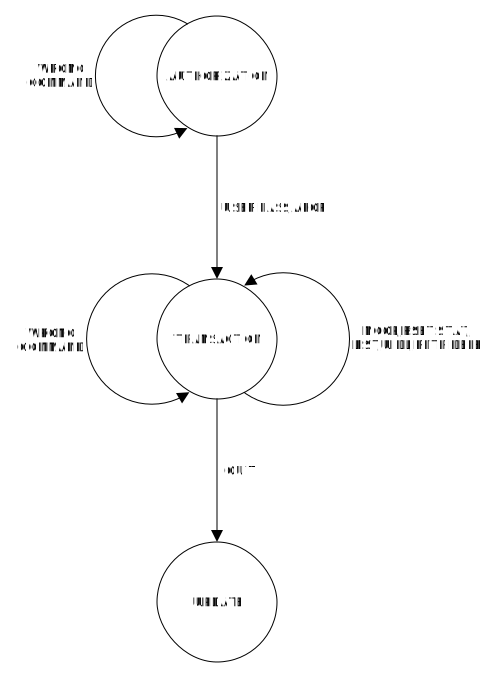
\includegraphics[scale=0.5]{images/FSM}
    \caption{Konečný automat pop3 servera}
	\label{IMG-FSM}
\end{figure}

\newpage %#########################################################################################

\makeatletter
\makeatother
\bibliographystyle{czechiso}
\begin{flushleft}
	\bibliography{quotation}
\end{flushleft}

\end{document} %###################################################################################


